%
% beispiele.tex %% Beispiele partieller Differentialgleichungen
%
% (c) 2008 Prof Dr Andreas Mueller
%
\chapter{Einf"uhrende Beispiele partieller Differentialgleichung\label{chapter-beispiele}}
\lhead{Einf"uhrende Beispiele}
In diesem Kapitel sollen einige Beispiele von Differentialgleichungen
dargestellt werden, die sp"ater zur Illustration der allgemeinen
Gesetze und der L"osungstechniken verwendet werden k"onnen.
Die Beispiele illustrieren
\begin{enumerate}
\item die vielf"altigen Anwendungen der Theorie der partiellen 
Differentialgleichungen,
\item drei grunds"atzlich verschiedene
Situationen, die jedoch alle in den Anwendungen auftreten, und
\item die Bedeutung und die m"oglichen Formen von Anfangs-
und Randbedingungen.
\end{enumerate}

\rhead{Wellengleichung}
\section{Wellengleichung}
\index{Wellengleichung}
In der einfachsten Form beschreibt diese Gleichung die Schwingungen der
Saite einer Gitarre oder eines Klaviers, oder der Lufts"aule eines
Blasinstrumentes.
\index{Klavier}
\index{Gitarre}
\index{Luftsaule@Lufts\"aule}
\index{Blasinstrument}
Nat"urlich ist sie auch anwendbar auf einen schwingenden
Balken, oder, in auf mehrere Dimensionen verallgemeinerter Form auf
schwingende Platten, die Schallausbreitung in einem Raum oder die Schwingungen
einer beliebigen dreidimensionalen Struktur.
\index{Balken}
\index{Platte}
Und selbstverst"andlich
lassen sich damit auch andere Wellen\-ph"a\-no\-mene modellieren:
elektromagnetische Wellen (Licht, Radio) oder flache Wellen an der
Wasseroberfl"ache.
\index{Welle!elektromagnetisch}
\index{Wasserwellen}

\subsection{Die Differentialgleichung der schwingenden Saite}
\index{Saite}
Eine d"unne Saite mit der linearen Massedichte $\mu$ sei zwischen den
Punkten $x=0$ und $x=l$ eingespannt. An den Enden der Saite wirkt eine
Kraft $F$. Wir suchen die Differentialgleichung, die die Bewegung der Saite
beschreibt, nachdem wir die Saite in eine bestimmte Form gebracht, und
zur Zeit $t=0$ losgelassen haben.

Offenbar k"onnen wir den momentanen Zustand der Saite mit Hilfe einer
Funktion $\psi(x,t)$ beschreiben, welche die Auslenkung der Saite
am Punkt $x$ zur Zeit $t$ angibt. Die L"osung des Problems besteht darin,
eine Differentialgleichung f"ur die Funktion $\psi$ zu finden.

Aus dieser Beschreibung des Problems k"onnen wir die Anfangsbedingungen zur
Zeit $t=0$ und die Randbedingungen f"ur alle Zeiten $t\ge 0$ bereits ableiten.
Zur Zeit $t=0$ ist die Form der Saite vorgegeben. Es gibt also eine Funktion
$f(x)$, welche nicht von der Zeit abh"angt, und die mindestens stetig
sein muss (weil die Saite sonst reisst). Die gesuchte L"osung $\psi$
muss erf"ullen:
\[
\psi(x,0)=f(x).
\]
Da die Saite sich an ihren Enden nicht bewegen kann, muss die Funktion
$\psi$ dort f"ur alle Zeiten den Wert $0$ haben:
\[
\psi(0,t)=\psi(l,t)=0\quad\forall t\ge 0.
\]

\begin{figure}
\begin{center}
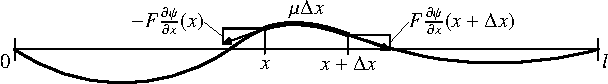
\includegraphics[width=\hsize]{images/saite-1}
\end{center}
\caption{Ableitung der Differentialgleichung der schwingenden Saite\label{saite}}
\end{figure}
F"ur die Ableitung der Bewegungsgleichung der Saite betrachten wir den
Ausschnitt zwischen $x$ und $x+\Delta x$ der Saite (Abbildung \ref{saite}).
Er hat die Masse
$\mu \Delta x$. F"ur die Beschleunigung dieses Abschnittes sind die
Kr"afte zust"andig, die senkrecht auf der $x$-Achse stehen. Die Kraft l"angs
der Seite ist nach Voraussetzung $F$, die Steigung gibt an, welcher Teil
dieser Kraft senkrecht auf die $x$-Achse wirkt. Insgesamt wirkt auf den
Abschnitt zwischen $x$ und $x+\Delta x$ die Kraft
\[
F\frac{\partial\psi}{\partial x}(x+\Delta x)-F\frac{\partial\psi}{\partial x}(x).
\]
Mit der Beschleunigung $\frac{\partial^2\psi}{\partial t^2}$ wird die
Bewegungsgleichung
\begin{align*}
\mu\Delta x\frac{\partial^2\psi}{\partial t^2}(x)&=
F\frac{\partial\psi}{\partial x}(x+\Delta x)-F\frac{\partial\psi}{\partial x}(x)\\
\Rightarrow\qquad
\frac{\mu}{F}\frac{\partial^2\psi}{\partial t^2}(x)&=
\frac1{\Delta x}\left(\frac{\partial\psi}{\partial x}(x+\Delta x)-\frac{\partial\psi}{\partial x}(x)\right)
\end{align*}
Geht man zum Grenzwert $\Delta x\to 0$ "uber, findet man die
partielle Differentialgleichung
\[
\frac{\partial^2\psi}{\partial t^2}=\frac{F}{\mu}\frac{\partial^2\psi}{\partial x^2}.
\]
Der Koeffizient $\frac{F}{\mu}$ hat die Dimension einer Geschwindigkeit im
Quadrat, es handelt sich um die Ausbreitungsgeschwindigkeit der Wellen entlang
der Saite.

\subsection{Die Differentialgleichung einer Orgelpfeife}
\index{Orgelpfeife}
\index{Luftdruck}
Grunds"atzlich ist die Analyse der schwingenden Saite auch auf
eine Orgelpfeife anwendbar. Die Rolle der Auslenkung "ubernimmt
hier der Luftdruck $p(x,t)$. Eine "ahnliche Argumentation wie bei
der schwingenden Saite f"uhrt uns erneut auf die Wellengleichung:
\[
\frac{\partial^2p}{\partial t^2}=
-a^2\frac{\partial^2p}{\partial x^2}
\]
Darin ist $a$ die Ausbreitungsgeschwindigkeit.

Die Randbedingungen sind jedoch etwas vielseitiger.
Ist die Pfeife am Ende geschlossen, man spricht von
einer gedackten Pfeife, kann sich die Luft an diesem Ende nicht bewegen.
Damit sich die Luft in Bewegung versetzt, muss ein Druckunterschied herschen,
die Beschleunigung der Luft ist proportional zum Druckgradienten
$\frac{\partial p}{\partial x}$. Umgekehrt muss als an Stellen, wo die
Luft sich gar nicht bewegen kann, der Druckgradient verschwinden.
Die Randbedingung am geschlossenen Ende ist daher
\[
\frac{\partial p}{\partial x}=0.
\]

Bei einer offenen Pfeife hingegen kann sich die Luft am Ende beliebig
bewegen, der Gradient kann daher jeden beliebigen Wert annehmen.
Anderseits kann man auch nicht fordern, dass der Druck am
Ende der Pfeife genau den Umgebungsdruck hat, da ja h"orbar eine
Schallwelle abgestrahlt wird, die genau diese Druckschwankungen am
Ende der Pfeife weitertransportiert. Allerdings sind diese Druckschwankungen
wesentlich geringer als die Druckschwankungen im inneren des Rohres.

Insgesamt erkennen wir, dass m"ogliche Randbedingungen f"ur dieses Problem
beliebig aus einer Bedingung an den Wert am Rand und einer Bedingung
an die Ableitung am Rand kombiniert werden kann.

\subsection{Wellengleichung in zwei und drei Dimensionen}
Analog zur Differentialgleichung einer schwingenden Saite kann
man auch die Differentialgleichung einer am Rand eingespannten Membran
ableiten.
\index{Membran}
Sei $G$ ein Gebiet in $\mathbb R^2$, und sei $\gamma$ der Rand
von $G$, $\gamma = \partial G$. Die Schwingungen einer entlang der Randkurve
$\gamma$ eingespannte Membran wird beschrieben durch eine Funktion
\[
\psi\colon G\times \mathbb R_{t \ge 0}\to\mathbb R\colon (x,y,t)\mapsto \psi(x,y,t)
\]
die die Auslenkung der Membran aus der Ruhelange angibt. Das Problem ist aber
erst bestimmt, wenn wir die Auslenkung der Membran zur Zeit $t=0$ kennen,
diese kann durch eine im Gebiet $G$ definierte Funktion $f(x,y)$ beschrieben
werden.

Die Funktion $\psi$
erf"ullt die Differentialgleichung
\[
\frac{\partial^2\psi}{\partial t^2}
=c^2\left(\frac{\partial^2\psi}{\partial x^2}+\frac{\partial^2\psi}{\partial y^2}\right),
\]
die Randbedingung
\[
\psi(x,y,t)=0\qquad \forall (x,y)\in\gamma,t\ge 0,
\]
und die Anfangsbedingung
\[
\psi(x,y,0)=f(x,y)\qquad \forall (x,y)\in G.
\]
Die Konstante $c$ ist die Ausbreitungsgeschwindigkeit der Wellen in der Membran.

In drei Dimensionen lautet
die Wellengleichung 
\[
\frac{\partial^2\psi}{\partial t^2}
=c^2\left(\frac{\partial^2\psi}{\partial x^2}
+\frac{\partial^2\psi}{\partial y^2}
+\frac{\partial^2\psi}{\partial z^2}
\right).
\]
Auch f"ur dieses Problem sind weitere Angaben notwendig, damit das Problem
wohl gestellt ist.
Zun"achst ist ein Gebiet $G\subset \mathbb R^3$ festzulegen, welches
eine geeignet glatte Randfl"ache hat.
Die L"osung $\psi(x,y,z,t)$ ist definiert f"ur Punkte $(x,y,z)\in G$
und f"ur Zeitpunkte $t\ge 0$.
Der Anfangszustand ist eine Funktion $f(x,y,z)$,
definiert auf $G$.

\subsection{Der Laplace-Operator}
In allen bisher diskutierten Problemen tritt der Laplace-Operator
\[
\Delta
=
\begin{cases}
\displaystyle
\frac{\partial^2}{\partial x^2}
+\frac{\partial^2}{\partial y^2}&\qquad\text{2 Dimensionen}\\
\\
\displaystyle
\frac{\partial^2}{\partial x^2}
+\frac{\partial^2}{\partial y^2}
+\frac{\partial^2}{\partial z^2}&\qquad\text{3 Dimensionen}
\end{cases}
\]
auf. Tats"achlich ist er bis auf einen konstanten Faktor der einzige Ausdruck
in den zweiten partiellen Ableitungen, der bei beliebigen Drehungen des
Koordinatensystems erhalten bleibt.

Tats"achlich zeigt sich in der Differentialgeometrie, dass der Laplace-Operator
eng mit der Geometrie des Raumes verkn"pft ist.

\section{Poisson-Problem}
\rhead{Poisson-Problem}

\subsection{Minimalfl"achen}
Welche Form nimmt eine Seifenhaut ein, die am Rande $\gamma$ eines
zweidimensionalen Gebietes $G$ auf die H"ohe $f(x,y)$ mit $(x,y)\in \gamma$
angehoben wird? Wir beschreiben die Seifenhaut durch eine Funktion
$\psi(x,y)$, nat"urlich muss gelten $\psi(x,y)=f(x,y)$ f"ur alle
Punkte $(x,y)\in\gamma$.
Im Gleichgewicht wird die Membran so geformt, dass die Kr"afte
der Oberfl"achenspannung sich an jeder Stelle der Seifenhaut gegenseitig
aufheben. Betrachtet man nur die $x$-Richtung, ist die Kraft auf die
Seifenhaut durch die zweite Ableitung in $x$-Richtung geben.
Diese Kraft muss durch Kraft kompensiert werden, die durch die
zweite Ableitung von $\psi$ in $y$-Richtung hervorgerufen wird.
Die Funktion $\psi$ muss also die Gleichung
\[
\frac{\partial^2\psi}{\partial x^2}+\frac{\partial^2\psi}{\partial y^2}
=\Delta\psi=0.
\]
Dieses einfache Argument ist auf den ersten Blick einleuchtend, br"auchte
aber eine noch etwas genauere Rechtfertigung. Darauf wollen wir allerdings
verzichten.

\subsection{Elektrisches Potential}
In der Elektrizit"atslehre wird gezeigt, dass das elektrostatische Feld 
ein Gradientenfeld ist. Der Gradient des Potentials $\varphi$  ist das
elektrische Feld:
\[
\vec E=\operatorname{grad}\varphi.
\]
Andererseits wird auch gezeigt, dass die Quellen des elektrische Feldes die
Ladungen sind, dass also insbesondere das elektrische Feld im Vakuum quellenfrei ist.
Die Divergenz von $\vec E$ muss also verschwinden, oder
\[
\operatorname{div}\vec E=\operatorname{div}\operatorname{grad}\varphi
=\Delta \varphi=0.
\]
Dies zeigt, dass wenigstens mathematisch ein enger Zusammenhang zwischen
einer gespannten Gummihaut und einem elektrischen Potential herrscht.
Als Modell f"ur ein Potential ist die Gummihaut daher eine bessere
N"aherung, als auf den ersten Blick scheinen mag.

\rhead{W"armeleitungsgleichung}
\section{W"armeleitungsgleichung}
\index{Warmeleitungsgleichung@W\"armeleitungslgleichung}
Die W"armeleitungsgleichung ist der Prototyp einer parabolischen partiellen
\index{Differentialgleichung!partielle!parabolische}
Differentialgleichung. Sie kann auch verwendet werden, um Diffusionsprozesse
zu beschreiben. L"asst man komplexe Werte der Konstanten zu, entpuppt
sie sich als sogar als die Grundgleichung der Quantenmechanik.

Wir leiten die W"armeleitungsgleichung im eindimensionalen Fall ab, und stellen
uns dazu einen w"armleitenden d"unnen Stab der L"ange $l$ vor. Punkte
entlang des Stabes haben die Koordinaten $x$ zwischen $0$ und $l$.
Die Temperaturverteilung in diesem Stab zur Zeit $t=0$ ist eine Funktion
$f(x)$. Wir suchen die Temperaturverteilung zu einem beliebigen sp"ateren Zeitpunkt.

Wir suchen also eine Funktion $T(x,t)$ und erwarten nat"urlich, dass sie
gen"ugend glatt ist, dass wird das Problem mit Hilfe einer partiellen
Differentialgleichung behandeln k"onnen. Die pro Zeiteinheit
durch der Querschnittsfl"ache an der Stelle $x$ fliessende W"armemenge ist
proportional zur Ableitung $\frac{\partial T}{\partial x}$.
Die W"armemenge im Teilst"uck zwischen $x$ und $x+\Delta x$ "andert sich also
pro Zeitenheit um einen Betrag, der proportional ist zu
\[
\frac{\partial T}{\partial x}(x+\Delta x)-\frac{\partial T}{\partial x}(x).
\]
Im Grenzwert $\Delta x\to 0$
"andert sich die Energiedichte also pro Zeiteinheit um einen zu
\[
\lim_{\Delta x\to 0}\frac1{\Delta x}\left(\frac{\partial T}{\partial x}(x+\Delta x)-\frac{\partial T}{\partial x}(x)\right)
=\frac{\partial^2T}{\partial x^2}
\]
proportionalen Betrag.
Die Temperatur ist aber propertional zur Energiedichte, also ist die "Anderung
der Energiedichte auch proportional zur "Anderung der Temperatur:
\[
\frac{\partial T}{\partial t}=a^2\frac{\partial^2T}{\partial x^2}.
\]
In der Physik lernt man, dass
\[
a=\sqrt{\frac{k}{c\varrho}},
\]
darin ist $k$ das W"armeleitverm"ogen, $c$ die spezifische W"arme
und $\varrho$ die Dichte.

Auch f"ur dieses Problem m"ussen Anfangs und Randbedingungen formuliert werden.
Als Anfangsbedinung wurde bereits die Funktion $f(x)$ vorgegeben, es muss
gelten
\[
T(x,0)=f(x)\qquad \forall x\in[0,l].
\]
Als Randbedingen kommen wiederum Bedingungen an die Temperatur oder an die
Ableitung am Rande in Frage.

Vorgabe der Temperatur an den Stellen $x=0$ und $x=l$ bedeutet physikalisch, dass
die Enden von einem externen W"armebad auf konstanter Temperatur gehalten
werden. Die Steigung von $T$ kann an dieser Stelle beliebige Werte annehmen,
sie gibt an, wie viel W"arme durch die Enden fliesst.

Vorgabe der Steigung an den Stellen $x=0$ und $x=l$ bedeutet physikalisch,
dass man den W"armefluss in oder aus dem Stab an dessen Enden vorgibt.

\rhead{"Uberschallstr"omung}
\section{"Uberschallstr"omung}
Im Jahre 1928 habilitierte sich Jakob Ackeret an der ETH mit einer
Schrift mit dem Titel ``"Uber Luft-Kr"afte bei sehr grossen
Geschwindigkeiten insbesondere bei ebenen Str"omungen''. Darin
zeigt er, wie mit einer linearen N"aherung die Luftkr"afte
in einer "Uberschallstr"omung berechnet werden k"onnen.
Die Geschwindigkeit des mit Geschwindigkeit $v_1$ in $x$-Richtung
anstr"omenden
Gases wird dabei als Gradient einer Funktion $\varphi$ gesucht,
es stellt sich heraus, dass die Funktion $\varphi$ die Gleichung
\[
(1-Ma_1)\frac{\partial^2\varphi}{\partial x^2}
+
\frac{\partial^2\varphi}{\partial y^2}
+
\frac{\partial^2\varphi}{\partial z^2}=0
\]
Dabei ist $Ma_1=\frac{v_1}{c_1}$, $c_1$ ist die Schallgeschwindigkeit.

F"ur kleine Geschwindigkeiten ist $(1-Ma_1)>0$, die Gleichung "ahnelt
der Poissongleichung. F"ur "Uberschallgeschwindigket ist jedoch
$(1-Ma_1) < 0$,
diese Differentialgleichung "ahnelt eher der Wellengleichung.
Wir k"onnen daraus bereits schliessen, dass mindestens in linearer
N"aherung das Str"omungsbild und auch die Luftwiderstandsverh"altnisse
sich grundlegend unterscheiden m"ussen.
Tats"achlich wird das Str"omungsbild im "Uberschallbereich dominiert
von den Schockwellen (Wellengleichung!), welche die Energie mit
Schallgeschwindigkeit vom umstr"omten K"orper wegtransportieren
(Abbildung~\ref{ueberschall2d}).

\rhead{Balkengleichung}
\section{Balkengleichung}
\index{Balken}
\index{Balkengleichung}
\index{Biegung}
Bei der Herleitung der Differentialgleichung einer Saite haben
wir verwendet, dass sich die Saite der Biegung nicht wiedersetzt.
Selbst eine beliebig starke Beigung hat keine Kraft zur Folge, die
die Biegung wieder strecken w"urde.
Ein Balken verh"alt sich jedoch ganz anders. Bei der Biegung entstehen
innere Spannungen im Material, welche den Balken wieder in die
gerade Ausgangslage zu bringen versuchen.
Wie diese Kr"afte entstehen, ist nicht Gegenstand dieser Vorlesung.
Es ist aber klar, dass die Spannungen umso gr"osser sein werden,
je gr"osser die Kr"ummung des Stabes ist. Sie sind auch proportional
zu einer Materialkonstanten, dem Elastizit"atsmodul $E$ und der
\index{Elastizitatsmodul@Elastizit\"atsmodul}
Gestalt des Querschnittes, ausgedr"uckt durch das Fl"achentr"agheitsmoment
\index{Flachentragheitsmoment@Fl\"achentr\"agheitsmoment}
$I$\footnote{Falls Ihnen das Fl"achentr"agheitsmoment nicht bekannt ist,
spielt das f"ur die weitere Diskussion keine Rolle.}.

Um die Gleichung eines schwingenden Stabes aufzustellen, brauchen wir
die Kr"afte, die den Balken in die Ruhelage zu bringen versuchen. Sei
$w(x,t)$ die Auslenkung des Balkens aus der Ruhelage zur Zeit $t$
und an der Stellen $x$. Der Balken soll die lineare Dichte $m$ haben.
Ein Element der L"ange $\Delta x$ des Balkens erf"ahrt dann die
folgenden Kr"afte:
\begin{enumerate}
\item R"ucktreibende Kr"afte durch die Spannung des Balkens: $-EI\frac{\partial^4}{\partial^4 x}w(t,x)\Delta x$
\item D"ampfung $-b\frac{\partial}{\partial t}w(t,x)\Delta x$
\item "Ausser Kr"afte (zum Beispiel Belastungen des Balkens) $q(x,t)\Delta x$
\end{enumerate}
Nach dem Newtonschen Gesetz m"ussen sich diese Kr"afte zu
\[
m\Delta x\frac{\partial^2}{\partial^2 t}w(t,x)
\]
summieren. Es gilt also pro Element des Balkens
\begin{align*}
m\frac{\partial^2}{\partial^2t}w(t,x)
&=-EI\frac{\partial^4}{\partial^4x}w(t,x)-b\frac{\partial}{\partial t}w(t,x)+q(t,x)
\\
EI\frac{\partial^4}{\partial^4x}w(t,x)
+b\frac{\partial}{\partial t}w(t,x)
+m\frac{\partial^2}{\partial^2t}w(t,x)
&=q(t,x)
\end{align*}
F"ur die Bewegung eines Balkens gilt also eine partielle Differentialgleichung.

\rhead{Plattengleichung}
\section{Plattengleichung}
\index{Plattengleichung}
Noch etwas komplizierter ist die Berechnung einer Platte. Im Gegensatz
zu einer Membran versuchen die Spannungen, die bei der Verbiegung der
Platte unter Last entstehen, die Platte wieder in die Ausgangslage zur"uck
zu bringen. Die Gleichung einer an der Stelle $(x,y)$ um den Betrag
$w(x,y)$ aus der $x$-$y$-Ebene ausgelenkten Platte ist
\[
D\left(
\frac{\partial^2}{\partial^2 x}
+
\frac{\partial^2}{\partial^2 y}
\right)
\left(
\frac{\partial^2}{\partial^2 x}
+
\frac{\partial^2}{\partial^2 y}
\right)
w(x,y)
=D\Delta\Delta w(x,y)
=p(x,y),
\]
wobei $D$ eine Materialkonstante ist und $p(x,y)$ der Druck, der
an der Stelle $(x,y)$ auf die Platte dr"uckt.

